\begin{frame}
\frametitle{Results: fuel demand}
% Here the reactor produces only hydrogen
\begin{columns}
    % Add figure with MTD fuel and UIUC Fleet fuel
    % Ideally I will put them on the same plot, but the x-axis is actually different
    \column[t]{5cm}
	\begin{figure}[htbp!]
		\begin{center}
			\includegraphics[height=6.2cm]{images/?}
		\end{center}
		\caption{.}
	\end{figure}

	\column[t]{5cm}
	% Add Diesel and E85 to this table
	\begin{table}[!htb]
		\centering
	    \caption{Hydrogen required and CO$_2$ produced by \gls{MTD} and \gls{UIUC} fleets.}
		\begin{tabular}{l|rr}
		\hline
	       & \textbf{MTD (Diesel)}   & \textbf{UIUC (Gasoline)}  \\ \hline
	       Daily (gal/day)    & 1,971.8        & 251.8            \\
	       Annual (gal/year)    & 719,717.6      & 91,925.1         \\ 
	    CO$_2$ (lbs/day)   & 44,129.5       & 4,945.3          \\
	    CO$_2$ (lbs/year)  & 16,107,279.9   & 1,805,408.9      \\ \hline
	       & \textbf{MTD ($H_2$)}   & \textbf{UIUC ($H_2$)}  \\ \hline
	    Daily H$_2$ (kg/day)    & 2,228.2        & 251.8            \\
	    Annual H$_2$ (kg/year)   & 813,280.9      & 91,925.1         \\\hline
		\end{tabular}
	    \label{tab:h2req}
	\end{table}
\end{columns}
\end{frame}


\begin{frame}
\frametitle{Results: Yearly Demand predictions}
\begin{columns}
    \column[t]{5cm}
	\begin{figure}[htbp!]
		\begin{center}
			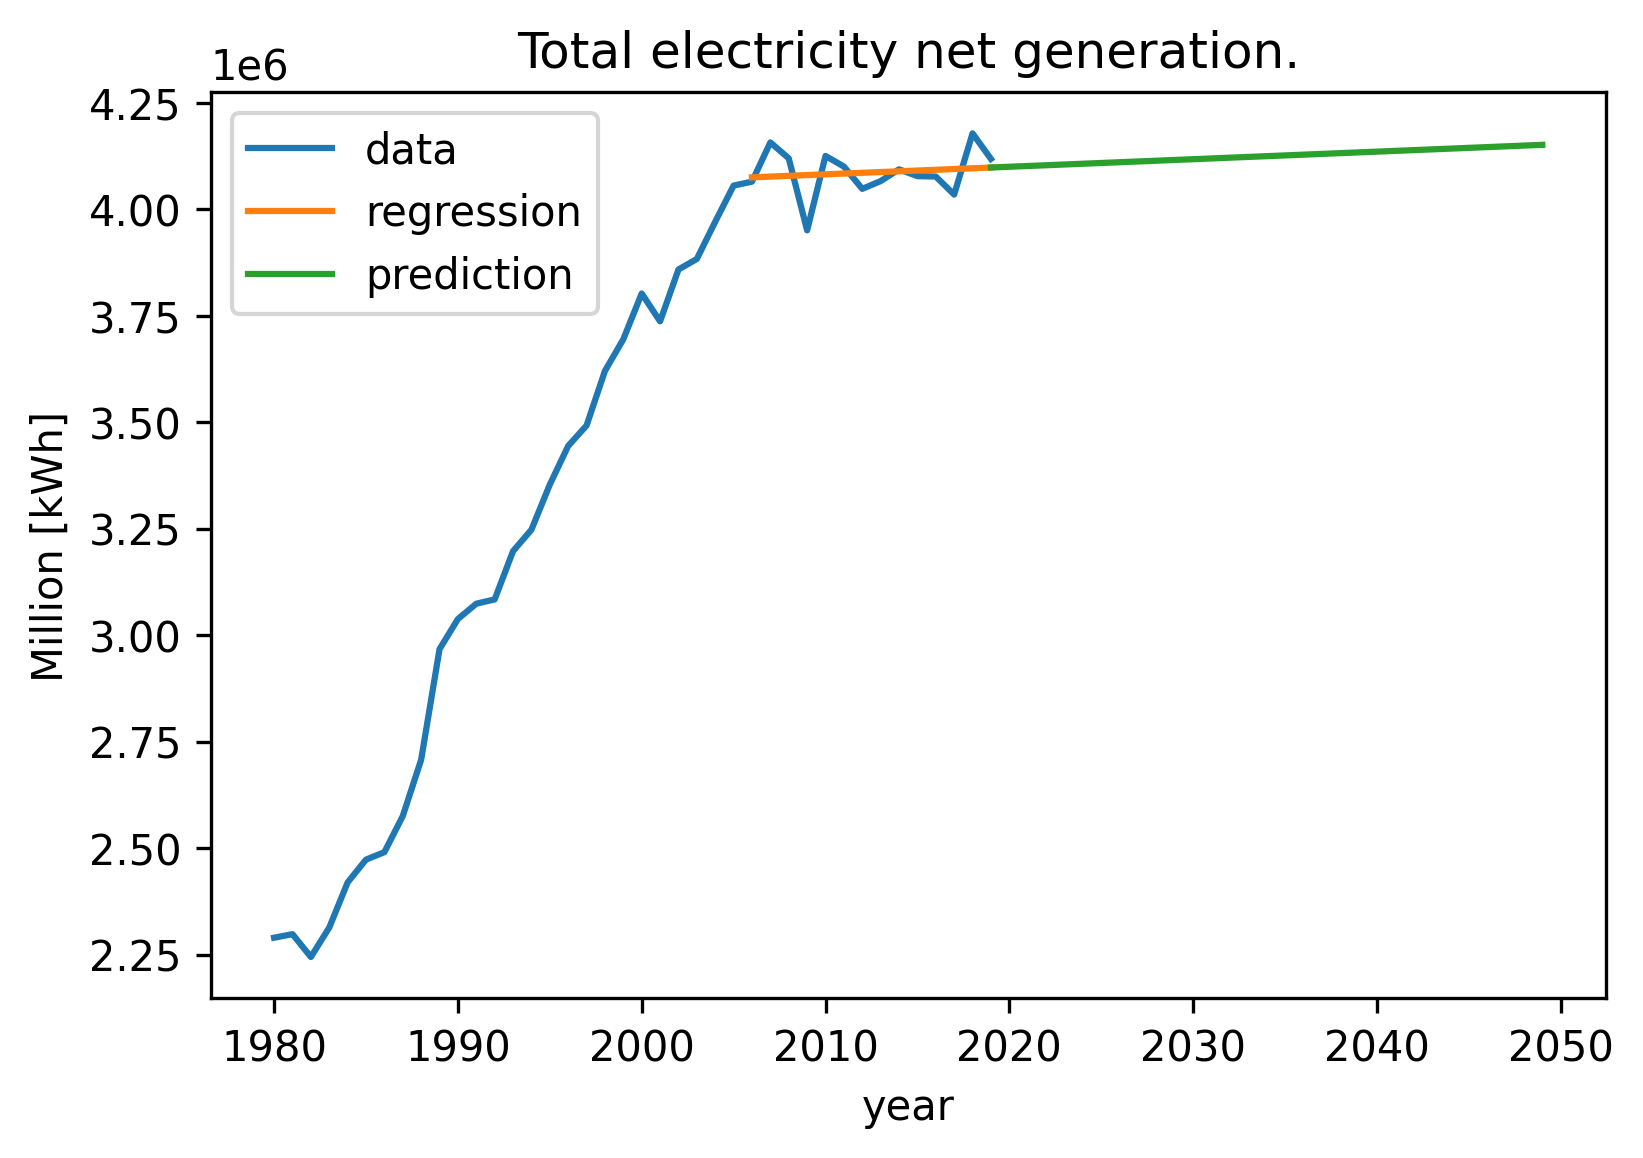
\includegraphics[height=6.2cm]{images/us-prediction1}
		\end{center}
		\caption{Prediction on the total electricity generation in the US for 2050.}
	\end{figure}

    \column[t]{5cm}
	\begin{figure}[htbp!]
		\begin{center}
			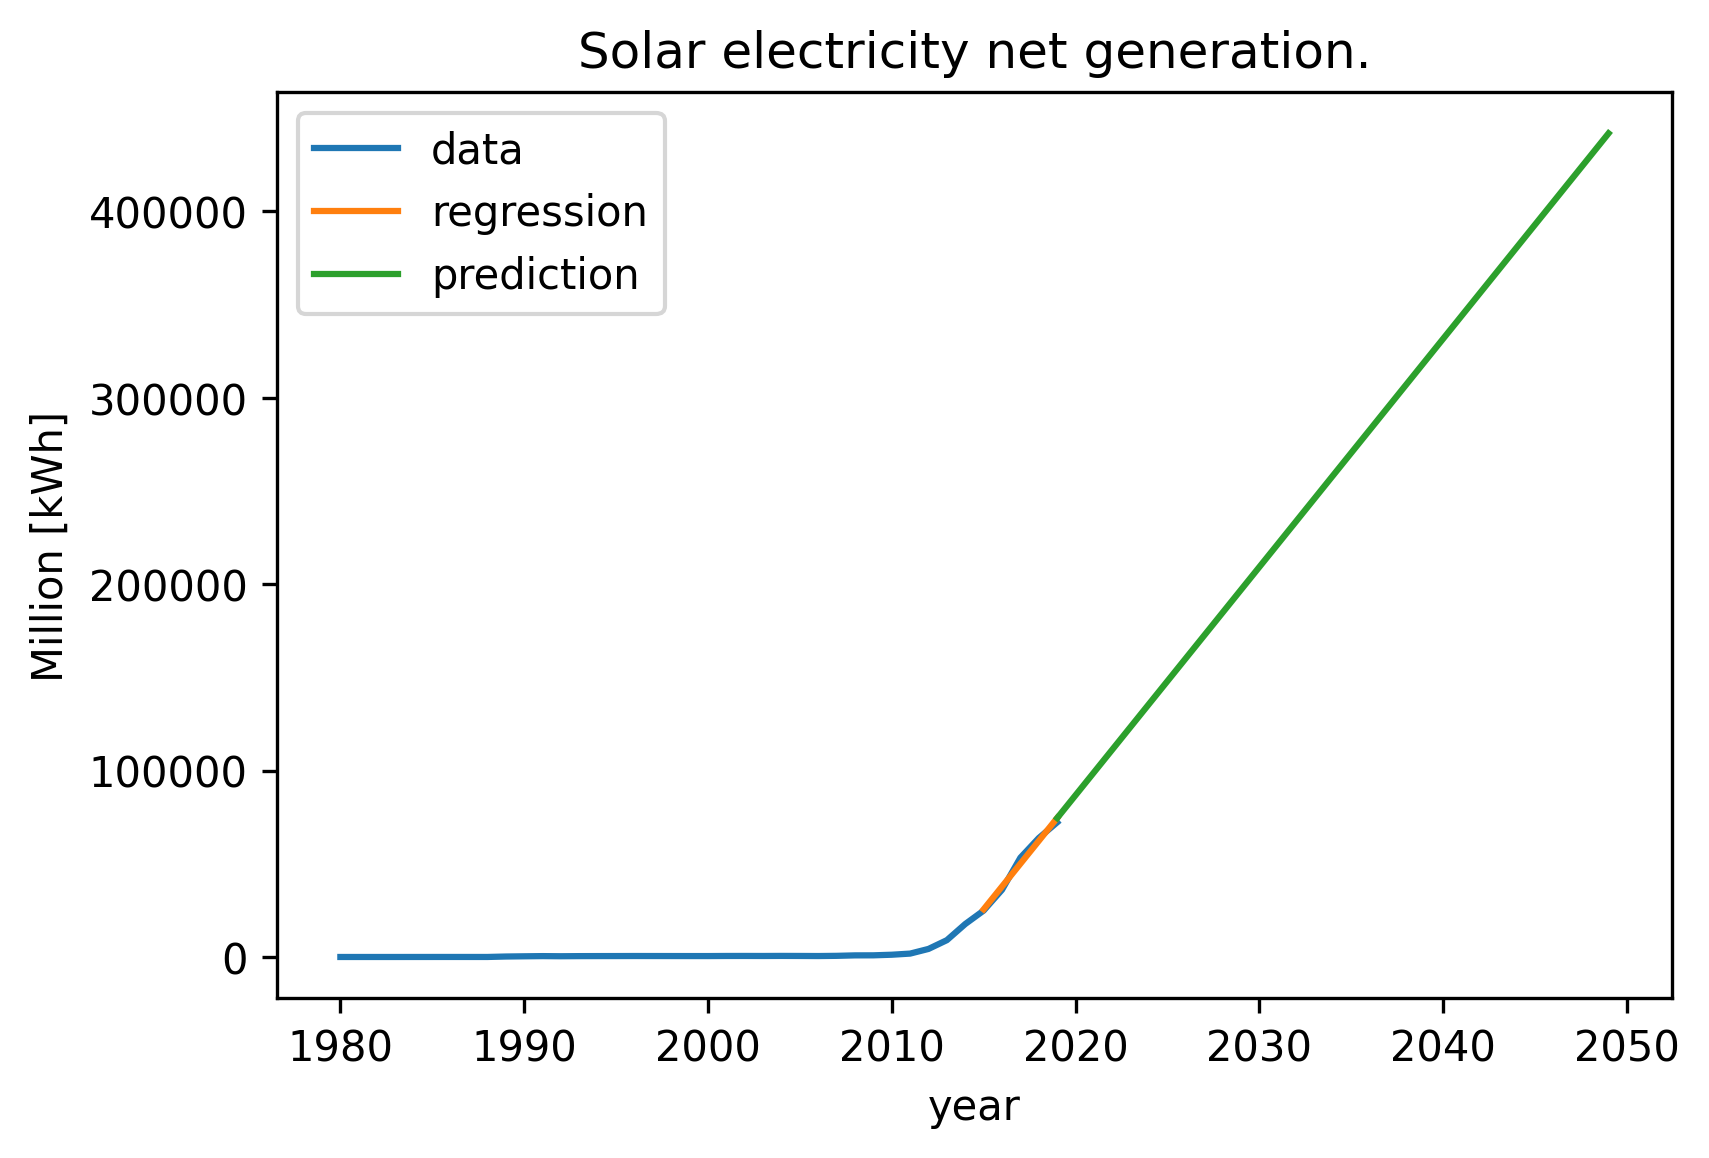
\includegraphics[height=6.2cm]{images/us-prediction2}
		\end{center}
		\caption{Prediction on the solar electricity generation in the US for 2050.}
	\end{figure}
\end{columns}
\end{frame}


\begin{frame}
\frametitle{Results: Hourly Demand predictions}
\begin{columns}
    \column[t]{5cm}
	\begin{figure}[htbp!]
		\begin{center}
			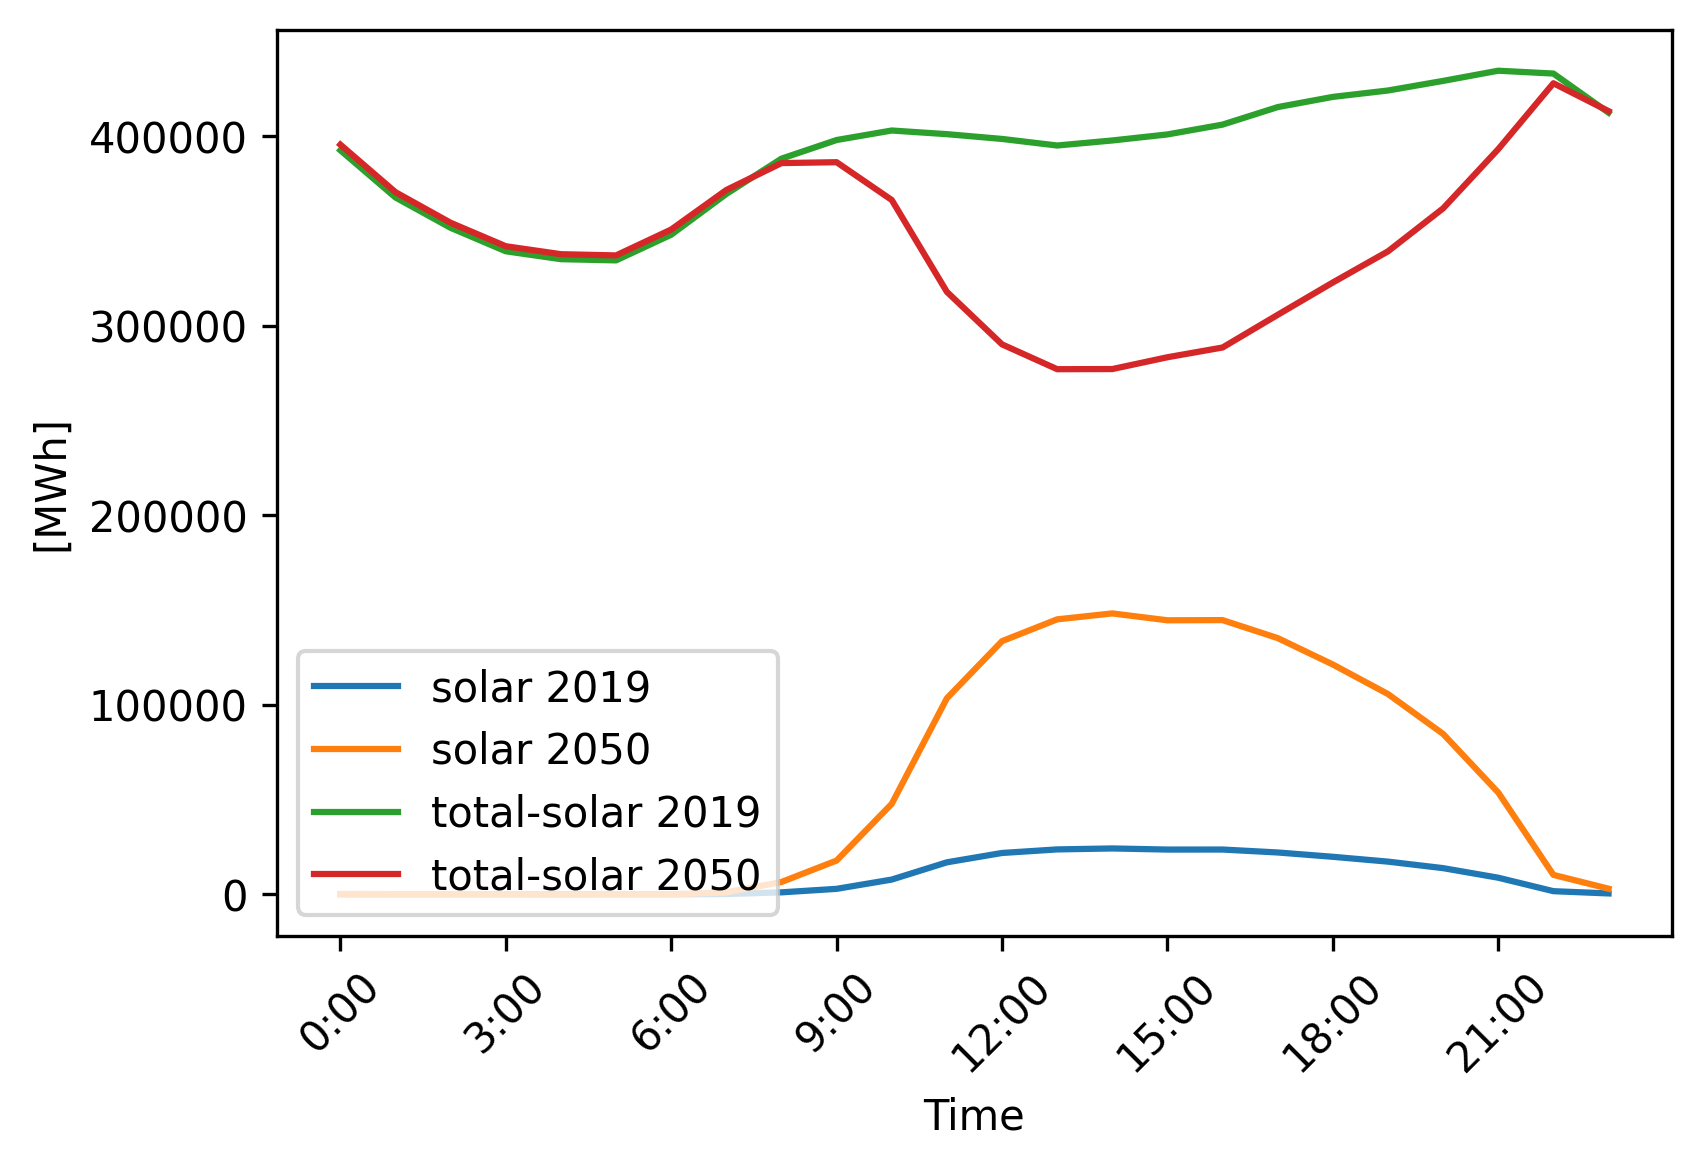
\includegraphics[height=6.2cm]{images/duck-curve4}
		\end{center}
		\caption{Prediction on US demand for 2050.}
	\end{figure}

    \column[t]{5cm}
	\begin{figure}[htbp!]
		\begin{center}
			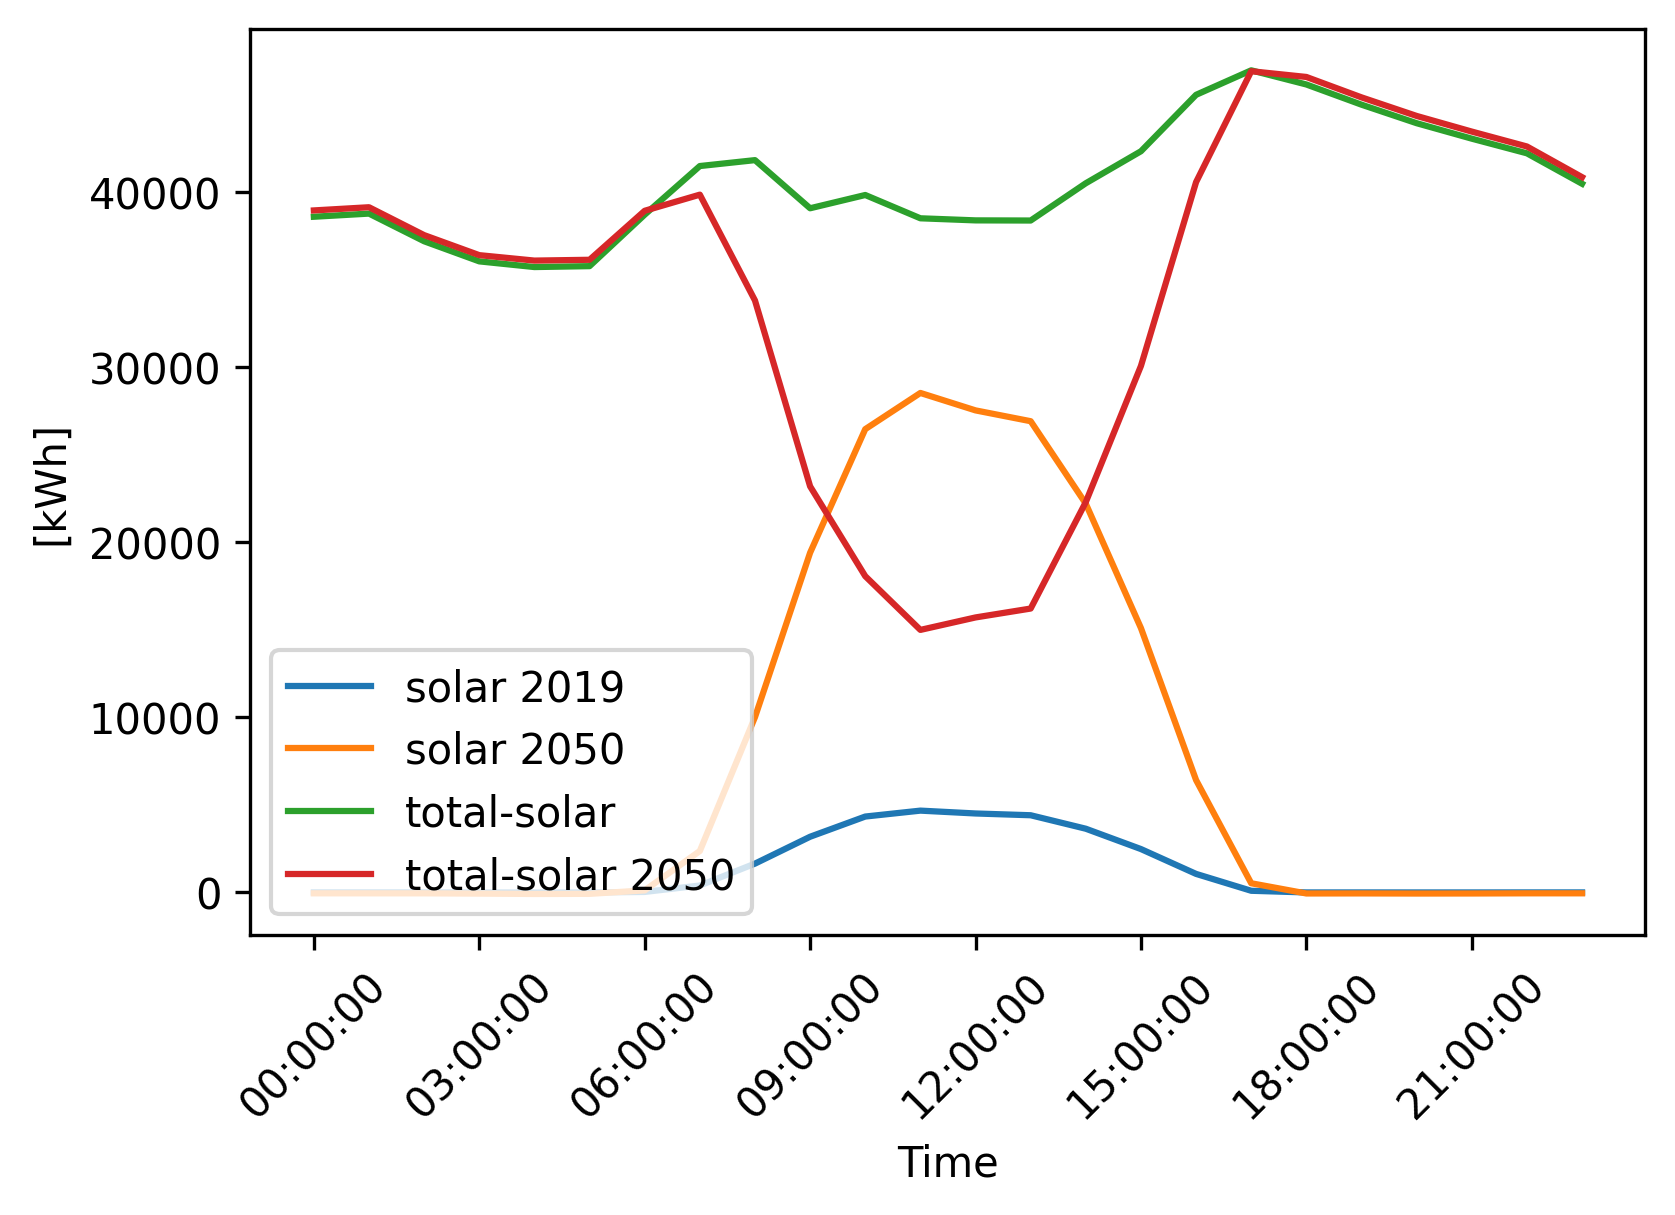
\includegraphics[height=6.2cm]{images/uiuc-duck}
		\end{center}
		\caption{Prediction on UIUC's demand for 2050.}
	\end{figure}
\end{columns}
\end{frame}


\begin{frame}
\frametitle{Results: Hydrogen for transportation}
\begin{columns}
    \column[t]{5cm}
	\begin{figure}[htbp!]
		\begin{center}
			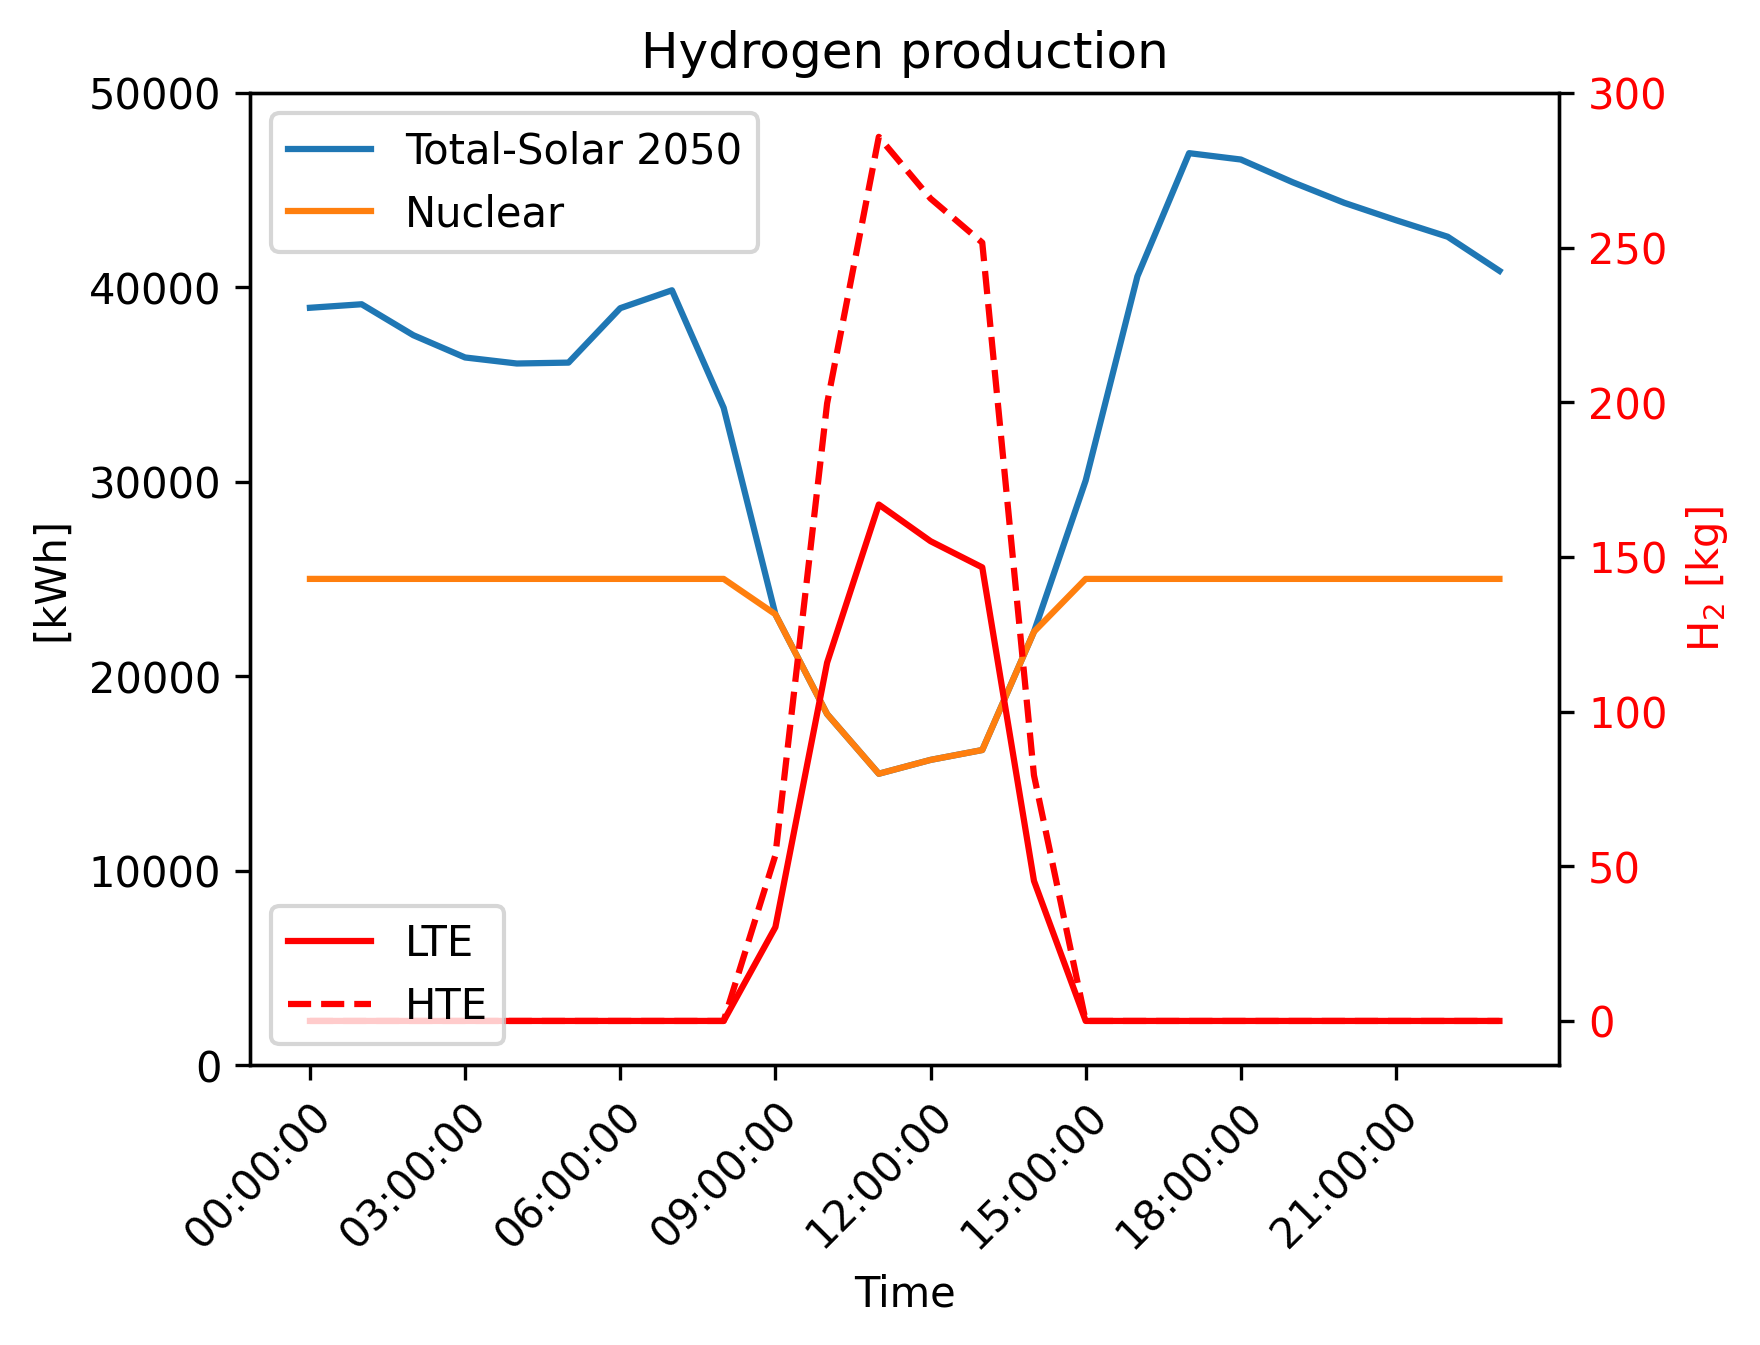
\includegraphics[height=6.2cm]{images/uiuc-hydro2}
		\end{center}
		\caption{Hydrogen production with the excess of energy.}
	\end{figure}

    \column[t]{5cm}

\end{columns}
\end{frame}


\begin{frame}
\frametitle{Results: Hydrogen for energy storage}
\begin{columns}
    \column[t]{5cm}
	\begin{figure}[htbp!]
		\begin{center}
			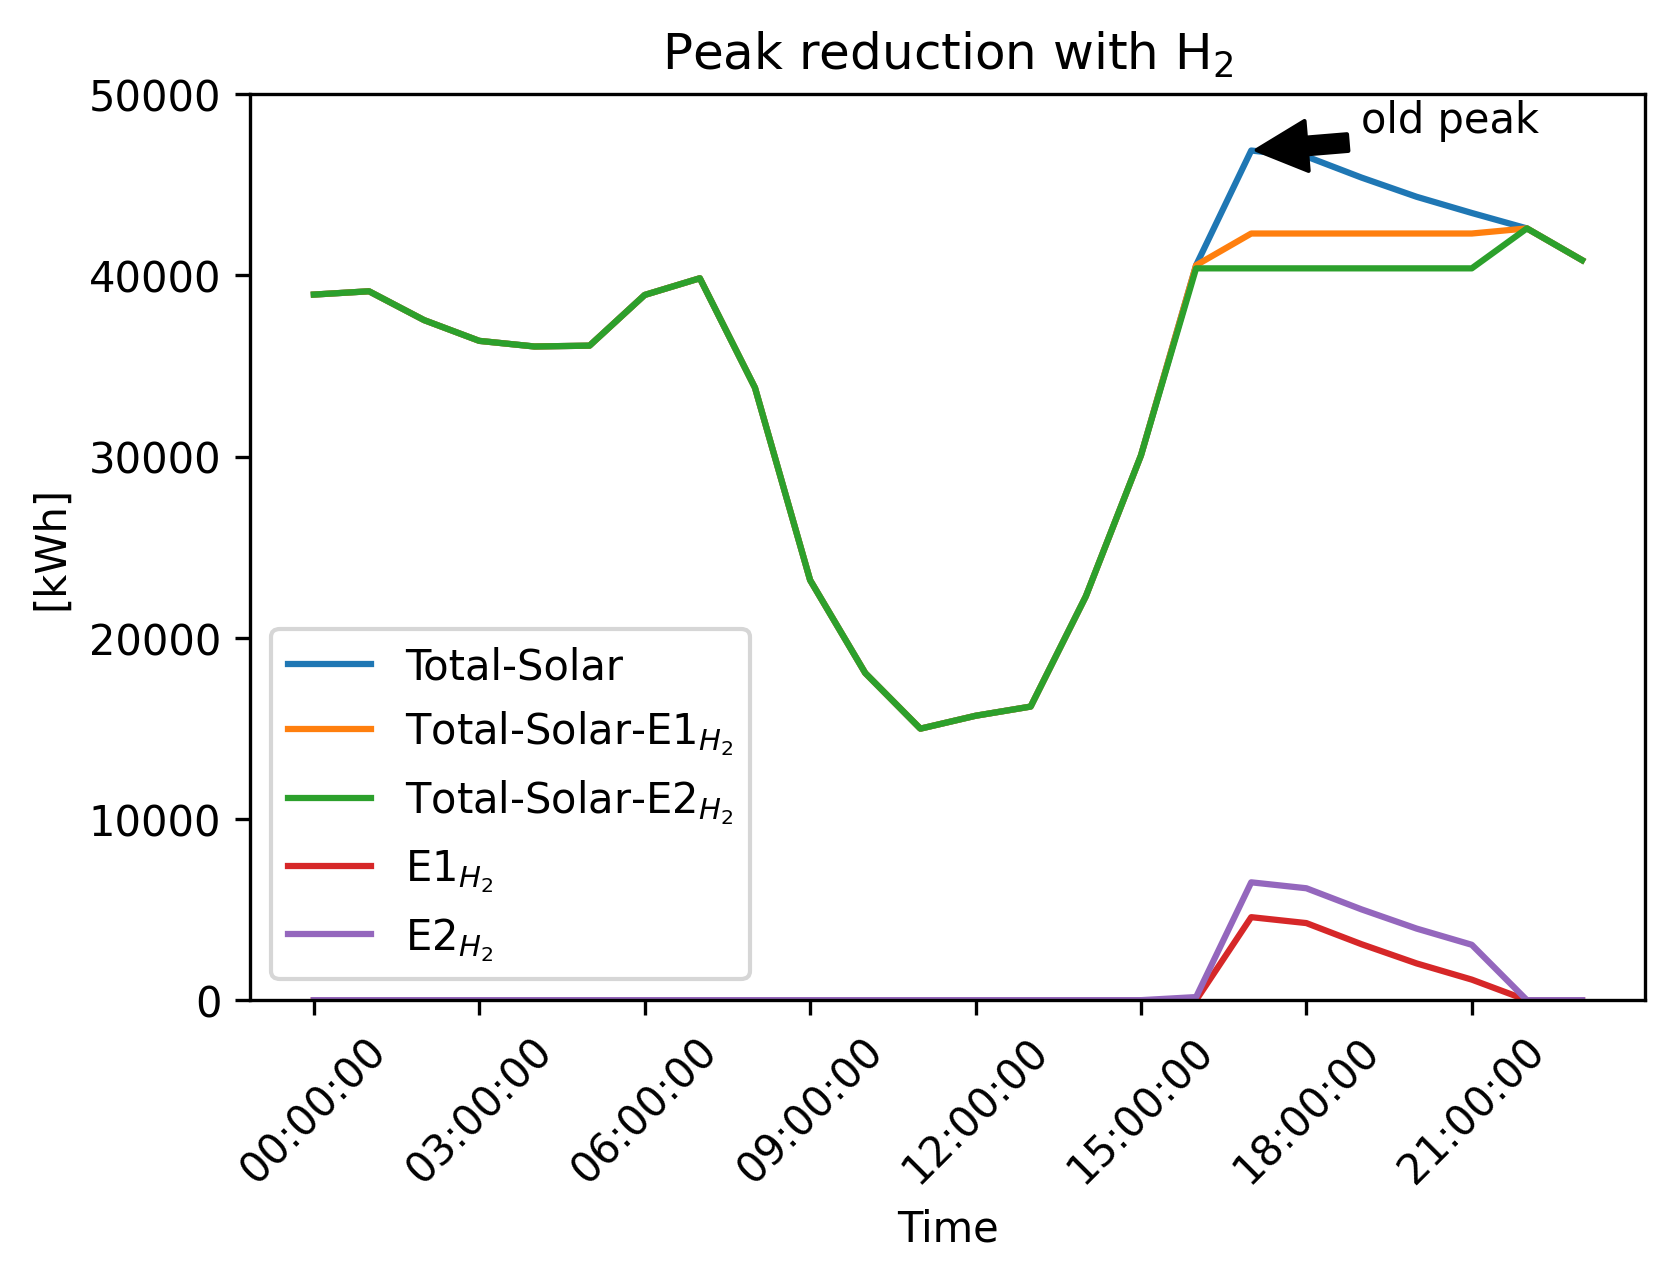
\includegraphics[height=6.2cm]{images/uiuc-hydro3}
		\end{center}
		\caption{Peak reduction by using the produced H$_2$.}
	\end{figure}

    \column[t]{5cm}

\end{columns}
\end{frame}